\section{Environment}
Because of the nature of the problem, we cannot use pre-existing datasets to train the agent. 
Rather, we configured a training environment to simulate Minesweeper games. In the environment,
\begin{itemize}
  \item a game represents an \textbf{episode},
  \item the board represents the \textbf{state}, and
  \item each possible move represents an \textbf{action}.
\end{itemize}
The first environment we used was a naive implementation, containing a basic 2D matrix representing the game board.
Each matrix value contained one of: a number from 0 to 8, corresponding to the number of adjacent mines; a $-$2, indicating an unopened cell; or $-$1, a mine.
The scope of possible actions is any cell -- imposing the possibility of selecting a previously-opened cell.
Because of this flaw, and the lack of penalization for repeated actions, the agent would often get stuck and fail to learn.
\\\\
A more advanced environment was implemented, restricting valid actions to only unopened cells.
The new environment also opens neighbouring cells when a safe cell is selected, in accordance with the real Minesweeper game.
These changes drastically reduced the number of steps taken to complete a game, making training both more efficient and more effective.
Additionally, in the new environment, if the first opened cell reveals a mine, the game will silently restart to avoid failing on the first move and not learning. 
This advanced environment was configured for use with both Q-learning and deep Q-learning.

\subsection{Reward Structure}
The initial reward structure (Structure 1) was brainstormed. Initially, the positively rewarded actions were winning a game, and opening a new cell and losing the game was a negative reward. When using such a simple reward structure with our very first environment (the most naive Gym environment), we found that even after 1000 runs, the agent failed to learn to not click on an already opened cell. This made sense as the reward structure was flawed, since reopening a cell would still result in the agent being positively rewarded. Hence, in our next version of the reward structure (Structure 2), we gave a negative reward to the agent for clicking on the already opened cell, and kept everything else the same as Structure 1.
\\\\
A more advanced reward structure (Structure 3) was then adapted to have the agent rewarded positively for winning and opening a new cell (strategically, based on what the agent has learnt so far). Structure 3 rewarded the agent negatively for guessing which cell to open, reopening an open cell, and losing.
\\\\
We did some research by actually playing the Minesweeper game, and observing someone who has never played the game to devise reward strategies that would help an agent learn more effectively. Based on that, we designed a new reward structure (Structure 4). Here, the agent was rewarded like in Structure 2, except in Structure 2 the reward for opening a new cell was a constant whereas in Structure 4, we decided to take a dynamic approach for opening a new cell. The new reward for opening a new cell was based on the percentage of new cells opened by the action - an action that chose a cell adjacent to a mine would be rewarded less than an action that would open neighbouring cells.
\\\\
Table 1 states the reward values for each action. The values are consistent throughout all four reward structures, except for the opening a cell action in Structure 4.

\begin{table}[h]
  \centering
  \begin{tabular}[t]{| l | c |}
    \hline
    \textbf{Action} & \textbf{Reward}\\
    \hline
    Opening a new cell \ \ & +0.3 \\
    Reopening a cell & -0.3 \\
    Guessing a cell & -0.3 \\
    Victory & +1.0 \\
    Loss & -1.0 \\
    \hline
  \end{tabular}
  \caption{Reward summary}
\end{table}


\subsubsection{Comparing Reward Structures}

We excluded Structure 1 from our tests, since we had already established the poor performance of the agent using that structure. 
\\\\
To compare the three remaining structures, we tested multiple episodes on different board sizes (Appendix A). The performance is judged based on the percentage of games won during testing. The overall results pointed towards the comparatively worse performance of Structure 4. However, the performance of Structure 2 and Structure 3 were relatively close.
\\\\
To further obtain the best structure to use, we compared Structure 2 and Structure 3. This time, we used a bigger board and more episodes for a deeper comparison. The results, as seen in the figures below, manifest that the agent trained with Structure 2 (which is one step simpler than Structure 3) was able to win a higher percentage of games consistently, even though not by a substantial difference. This could potentially mean that Structure 3 is overcomplicating the reward structure, and trying harder to control the agent does not lead to better results.

\begin{figure}[H]
\centering
\makebox[\textwidth]{
	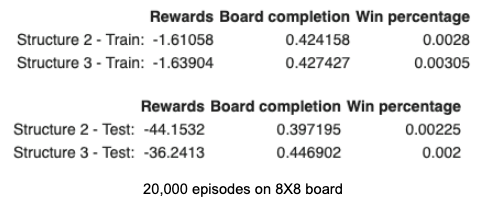
\includegraphics[width=0.55\textwidth]{reward-20k.png}
	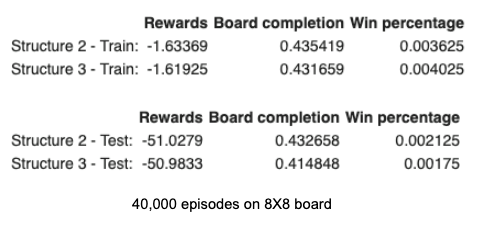
\includegraphics[width=0.55\textwidth]{reward-40k.png}
}
\caption{Comparison of Structure 2 and Structure 3}
\end{figure}

Since Structure 2 performed better when tested, we chose to train our Q-learning and deep Q-learning agents using this structure. Recall that this structure positively rewarded for winning (+1) and opening a new cell (+0.3), and negatively rewarded for losing (-1) and reopening an already opened cell (-0.3).
